\begin{figure*}[p]
\centering
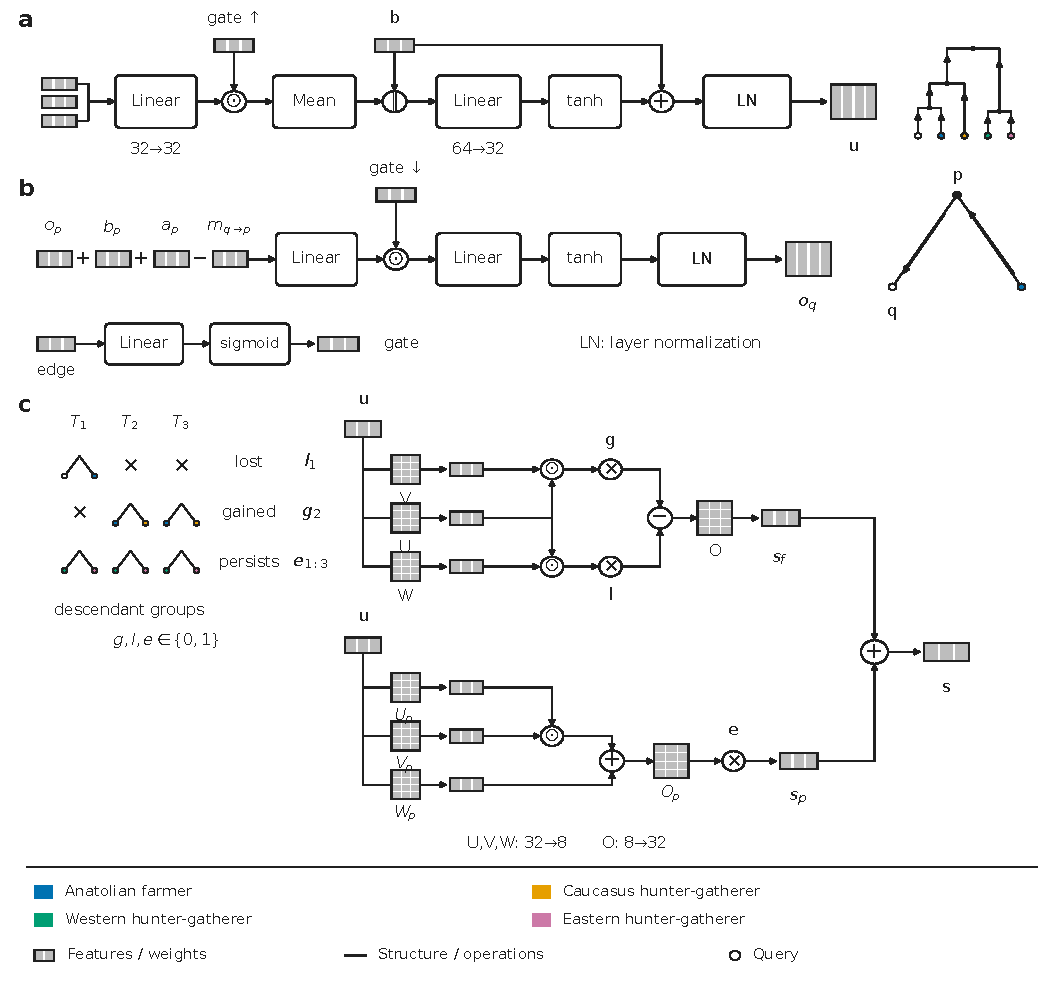
\includegraphics[width=\textwidth]{figures/TreeLoom_operators.pdf}
\caption{\textbf{a,} Upward node update. Each child state passes through a linear map and its edge gate. Their arithmetic mean joins the node input $b$, then passes through a linear map, tanh, a residual addition and layer normalization. This operation repeats from leaves to root.
\textbf{b,} Downward node update. Parent outside state $o_p$, input $b_p$ and mean child message $a_p$ are combined, excluding the recipient's normalized contribution $m_{q\to p}$. Two linear maps, an edge gate, tanh and normalization produce the child's outside state. This repeats from root to leaves, starting with zero outside state at the root. Edge features generate each directional gate through a linear map and sigmoid.
\textbf{c,} Structural corrections encode changes in descendant groups. Descendant groups appear, disappear or persist across trees. Binary flags select two factored transformations of the current upward state $u$. The examples mark loss at $T_1$, gain at $T_2$ and persistence across all three trees. Neighboring hidden states do not enter these circuits. Matrices have separate weights between the two corrections. The symbol $\odot$ is elementwise multiplication, $\parallel$ is concatenation, and $\times$ multiplies by a scalar. Diagram state $u$ is the upward state $h_v$ in the equations.}
\label{fig:operators}
\end{figure*}
